\documentclass{report}
\usepackage[T1]{fontenc} % Fontes T1
\usepackage[utf8]{inputenc} % Input UTF8
\usepackage[backend=biber, style=ieee]{biblatex} % para usar bibliografia
\usepackage{csquotes}
\usepackage[portuguese]{babel} %Usar língua portuguesa
\usepackage{blindtext} % Gerar texto automaticamente
\usepackage[printonlyused]{acronym}
\usepackage{hyperref} % para autoref
\usepackage{graphicx}
\usepackage{indentfirst}
\usepackage{float} % para posicionamento de imagens

\bibliography{bibliografia}


\begin{document}

% Definições

\def\titulo{A ERA DA INTELIGÊNCIA ARTIFICIAL}
\def\data{10 de novembro de 2023}
\def\repositorio{Repositório no GitHub: \\ infor2023-ap-g-infor2023-ap-g59}
\def\autores{Matilde Marabuto, Francisco Pedreiras}
\def\autorescontactos{(118866) matilde.morais@ua.pt, (119781) flrp@ua.pt}
\def\versao{VERSÃO 2}
\def\departamento{Dept. de Eletrónica, Telecomunicações e Informática}
\def\empresa{Universidade de Aveiro}
\def\logotipo{ua.pdf}
%
%%%%%% CAPA %%%%%%
%
\begin{titlepage}

\begin{center}
%
\vspace*{50mm}
%
{\Huge \titulo}\\
%
\vspace{10mm}
%
{\Large \empresa}\\
%
\vspace{10mm}
%
{\LARGE \autores}\\ 
%
\vspace{30mm}
%
\begin{figure}[h]
\center
\includegraphics{\logotipo}
\end{figure}
%
\vspace{30mm}
\end{center}
%
\begin{flushright}
\versao
\end{flushright}
\end{titlepage}

%%  Página de Título %%
\title{%
{\Huge\textbf{\titulo}}\\
{\Large \departamento\\ \empresa\\}
}
%
\author{%
    \autores \\
    \autorescontactos \\ \\
    \repositorio
}
%
%
\date{10 de novembro de 2023}
%
\maketitle

\pagenumbering{roman}

%%%%%% RESUMO %%%%%%
\begin{abstract}

	Este relatório aborda o tema da Era da \ac{ia}, realçando a sua evolução histórica, os seus usos contemporâneos e expectativas futuras. A \ac{ia} mexe com a forma como vivemos e trabalhamos, realizando tarefas que anteriormente seriam reservadas ao Homem. O relatório averigua a definição de \ac{ia}, o seu passado, desde a máquina de Turing até sitemas como o \textit{ChatGPT}, abrangendo fenômenos como o programa \textit{Logic Theorist} e a robô \textit{SOPHIA}.

	Os tipos de \ac{ia}, como fraca e forte, \ac{ml} e \ac{ia} Quântica, são desenvolvidos, tal como a rápida expansão destas ferramentas, impulsionada pelo incremento da capacidade computacional e arquiteturas de \textit{hardware} especializadas. Os usos atuais da \ac{ia} nas áreas da saúde, educação, assistência virtual e finanças são comentados, apresentando vantagens como diagnósticos médicos mais exatos e aconselhamento financeiro caracterizado.

	As vantagens da \ac{ia} tratadas incluem automatização eficiente, atenuação de erros humanos e processamento de maiores volumes de dados, enquanto que nas desvantagens são abordadas questões de ética, tendências nos algoritmos e implicâncias com privacidade e segurança de dados. O relatório aborda a receita do mercado da \ac{ia}, demonstrando o seu crescimento veloz.

	Conclusivamente, a \ac{ia} é apresentada como um recurso renovador, porém com os seus desafios éticos e uma urgente necessidade de regulamentação. As perspetivas futuras para este contêm avances tecnológicos, o seu uso em diversos setores do sociedade, repercussão no mercado de trabalho e a necessidade de inovação contínua e trabalho cooperativo internacional.
	
\end{abstract}

\renewcommand{\contentsname}{Índice}
\tableofcontents
% \listoftables     % descomentar se necessário
\listoffigures


%%%%%%%%%%%%%%%%%%%%%%%%%%%%%%%
\clearpage
\pagenumbering{arabic}

%%%%%%%%%%%%%%%%%%%%%%%%%%%%%%%%
\chapter{Introdução}
\label{chap.introducao}

	A \ac{ia} é uma ferramenta revolucionária, representada através da ciência da computação, que se centra no desenvolvimento de algoritmos e sistemas que têm o potencial de transformar a maneira como vivemos e trabalhamos, uma vez que podem realizar tarefas que exigeriam interferência humana.
		
	O acelerado avanço deste recurso suscita dúvidas e desafios, desde questões de ética e privacidade ao impacto que este pode ter na sociedade. 
		
	O crescimento desta tecnologia foi de tal forma exponencial que, desde a \textit{app Waze} ás \ac{avs}, como, por exemplo, a \textit{Siri} e a \textit{Alexa}, atualmente, vários programas utilizam esta ferramenta.
	
	Este relatório pretende contextualizar a \ac{ia} na história, demonstrar a sua evolução e a grande importância que tem no dia-a-dia. Ainda temos como objetivo elucidar as vantagens e desvantagens do seu uso, em várias situações.
	
	Após esta introdução, a \autoref{sec.o_que_e_a_ia} abordará a definição de \ac{ia}, seguido pela sua história, na \autoref{subsec.a_historia_da_ia}. A \autoref{subsec.os_tipos_de_ia}, \autoref{sec.a_rapida_explosao_da_ia} e \autoref{sec.os_usos_atuais_da_ia} abordarão, sequencialmente, os tipos de \ac{ia}, a rápida explosão desta tecnologia e os seus usos atuais. As vantagens e desvantagens, respetivamente, serão debatidas na \autoref{subsec.vantagens} e \autoref{subsec.desvantagens}. Na \autoref{sec.o que esperar}, serão discutidas as expectativas para o futuro da \ac{ia}. Por fim, os \autoref{chap.analise} e \autoref{chap.conclusao} contarão com a análise e conclusões finais.

\chapter{A Inteligência Artificial}
\label{chap.a_inteligencia_artificial}

\section{O que é a IA?}
\label{sec.o_que_e_a_ia}

	A \ac{ia} é uma ferramenta transformadora, representada através da ciência da computação, que se centra no desenvolvimento de algoritmos e sistemas que têm o potencial de transformar a maneira como vivemos e trabalhamos, uma vez que podem realizar tarefas que, de outra forma, exigeriam interferência humana.

	De acordo com o artigo \textit{"O que é a inteligência artificial e como funciona?"}, publicado pelo Parlamento Europeu, em 2020, a \ac{ia} é “a capacidade de uma máquina reproduzir competências humanas, como é o caso do raciocínio, a aprendizagem, o planeamento e a criatividade". \cite{artigo}

	O desenvolvimento desta tecnologia possui um vasto leque de abordagens, entre as quais o \ac{ml}, no qual os algoritmos são escritos para que estes reconheçam padrões, efetuem previsões e aprendam como lidar com a situação que lhes é apresentada, como é o caso, por exemplo, do \textit{ChatGPT}, jogos de xadrez e ainda carros de condução autónoma.
	
\begin{figure}[H]
\caption{\textit{ChatGPT}}
\centering
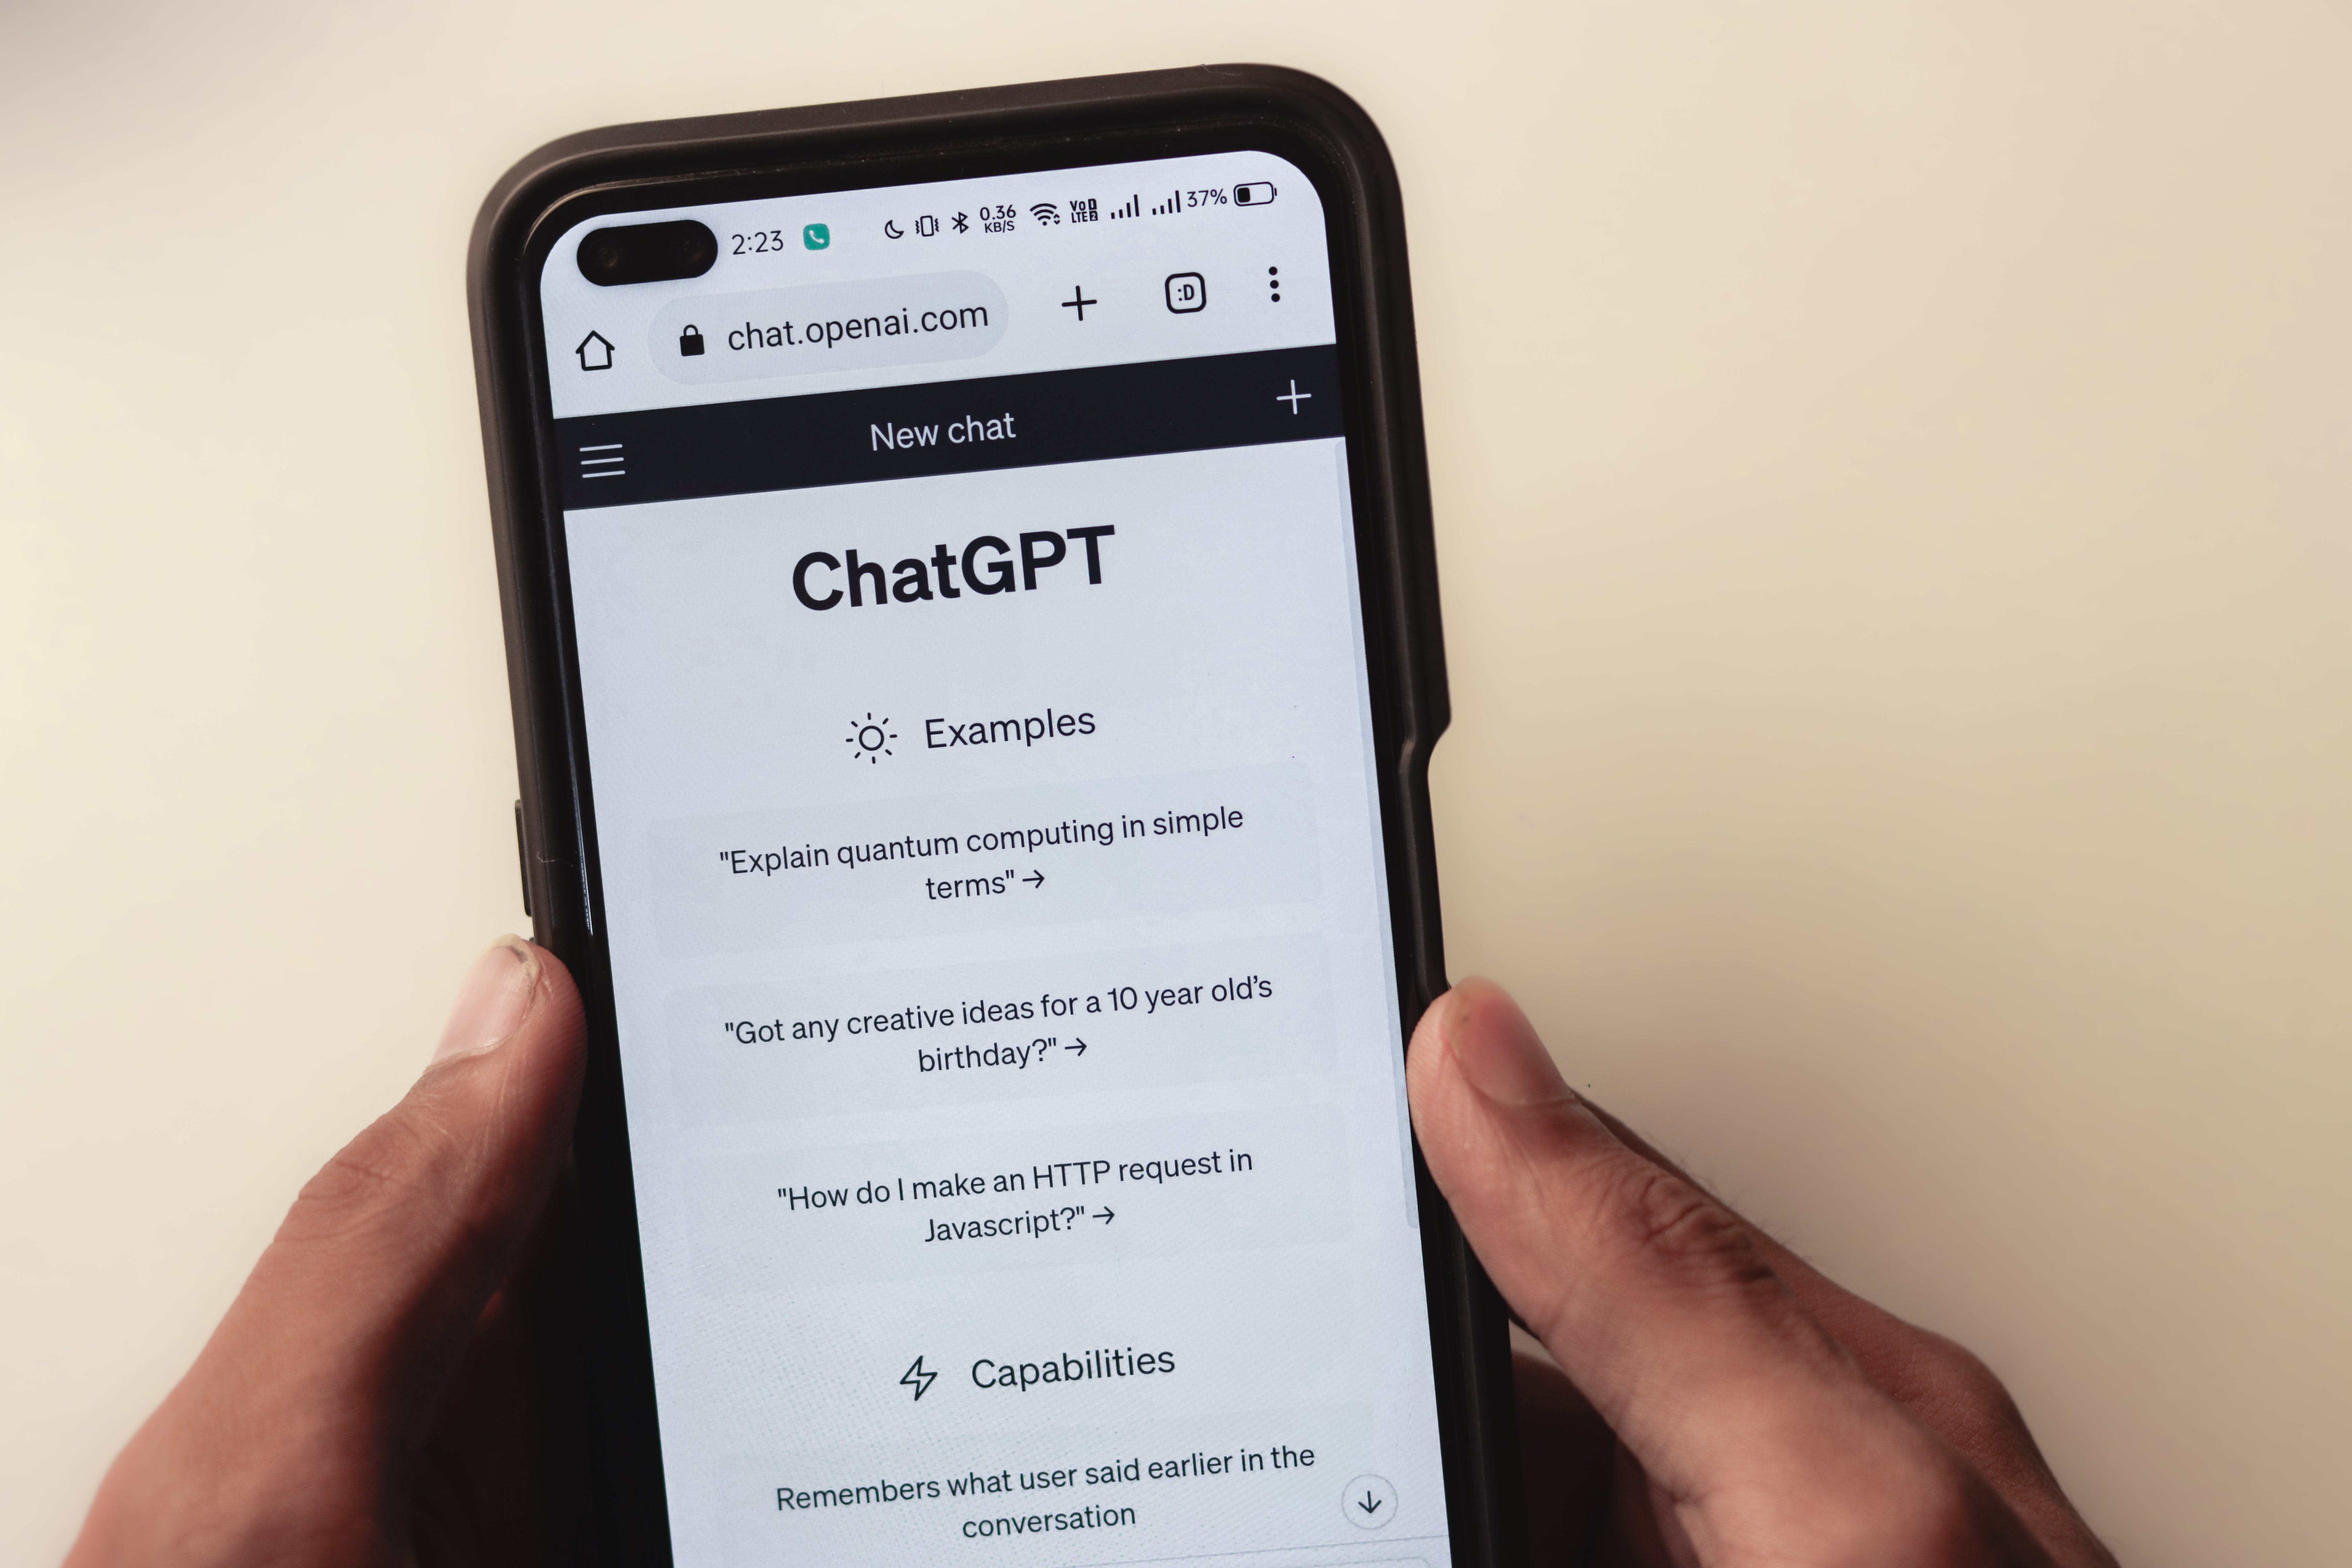
\includegraphics[width=8cm]{imagens/chatgpt.jpg}
\label{chatgpt}
\end{figure}

\nocite{chatgpt}

\subsection{A história da IA}
\label{subsec.a_historia_da_ia}

	Apesar de nos dias de hoje o tema da \ac{ia} ser muito popular, esta porção da ciência é a realização de um sonho do Homem, com raízes em mitos, ideias e histórias que exploram a criação de seres artificiais com capacidades inteligentes, de forma semelhante ao ser humano.
	
\begin{figure}[H]
\caption{Crescimento da receita da \ac{ia} corporativa, em milhares de dólares (US), ao longo dos anos}
\centering
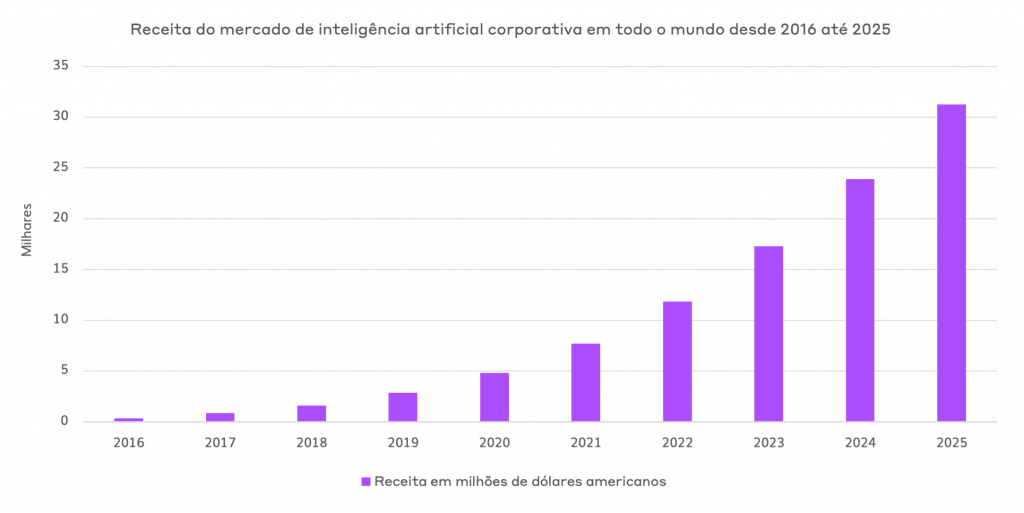
\includegraphics[width=8cm]{imagens/grafico3.png}
\label{Crescimento da receita de IA em milhares de dolares ao longo dos anos}
\end{figure}

\nocite{grafico3}

	O primeiro grande passo para a criação desta tecnologia foi dado pelo matemático inglês Alan Turing, conhecido como o pai da computação. Durante a 2ª Guerra Mundial, o matemático concebeu a ideia da máquina de Turing, que permitiria, mais tarde, realizar qualquer cálculo que fosse descrito por um algoritmo.

	O verdadeiro impulso para a criação do primeiro campo de pesquisa focado no desenvolvimento da \ac{ia} só foi dado em 1956, quando um conjunto de cientistas desenvolveram o primeiro programa deste tipo, denominado \textit{Logic Theorist}, durante uma conferência, no campus Darthmouth College.

\begin{figure}[H]
\caption{Dartmouth College}
\centering
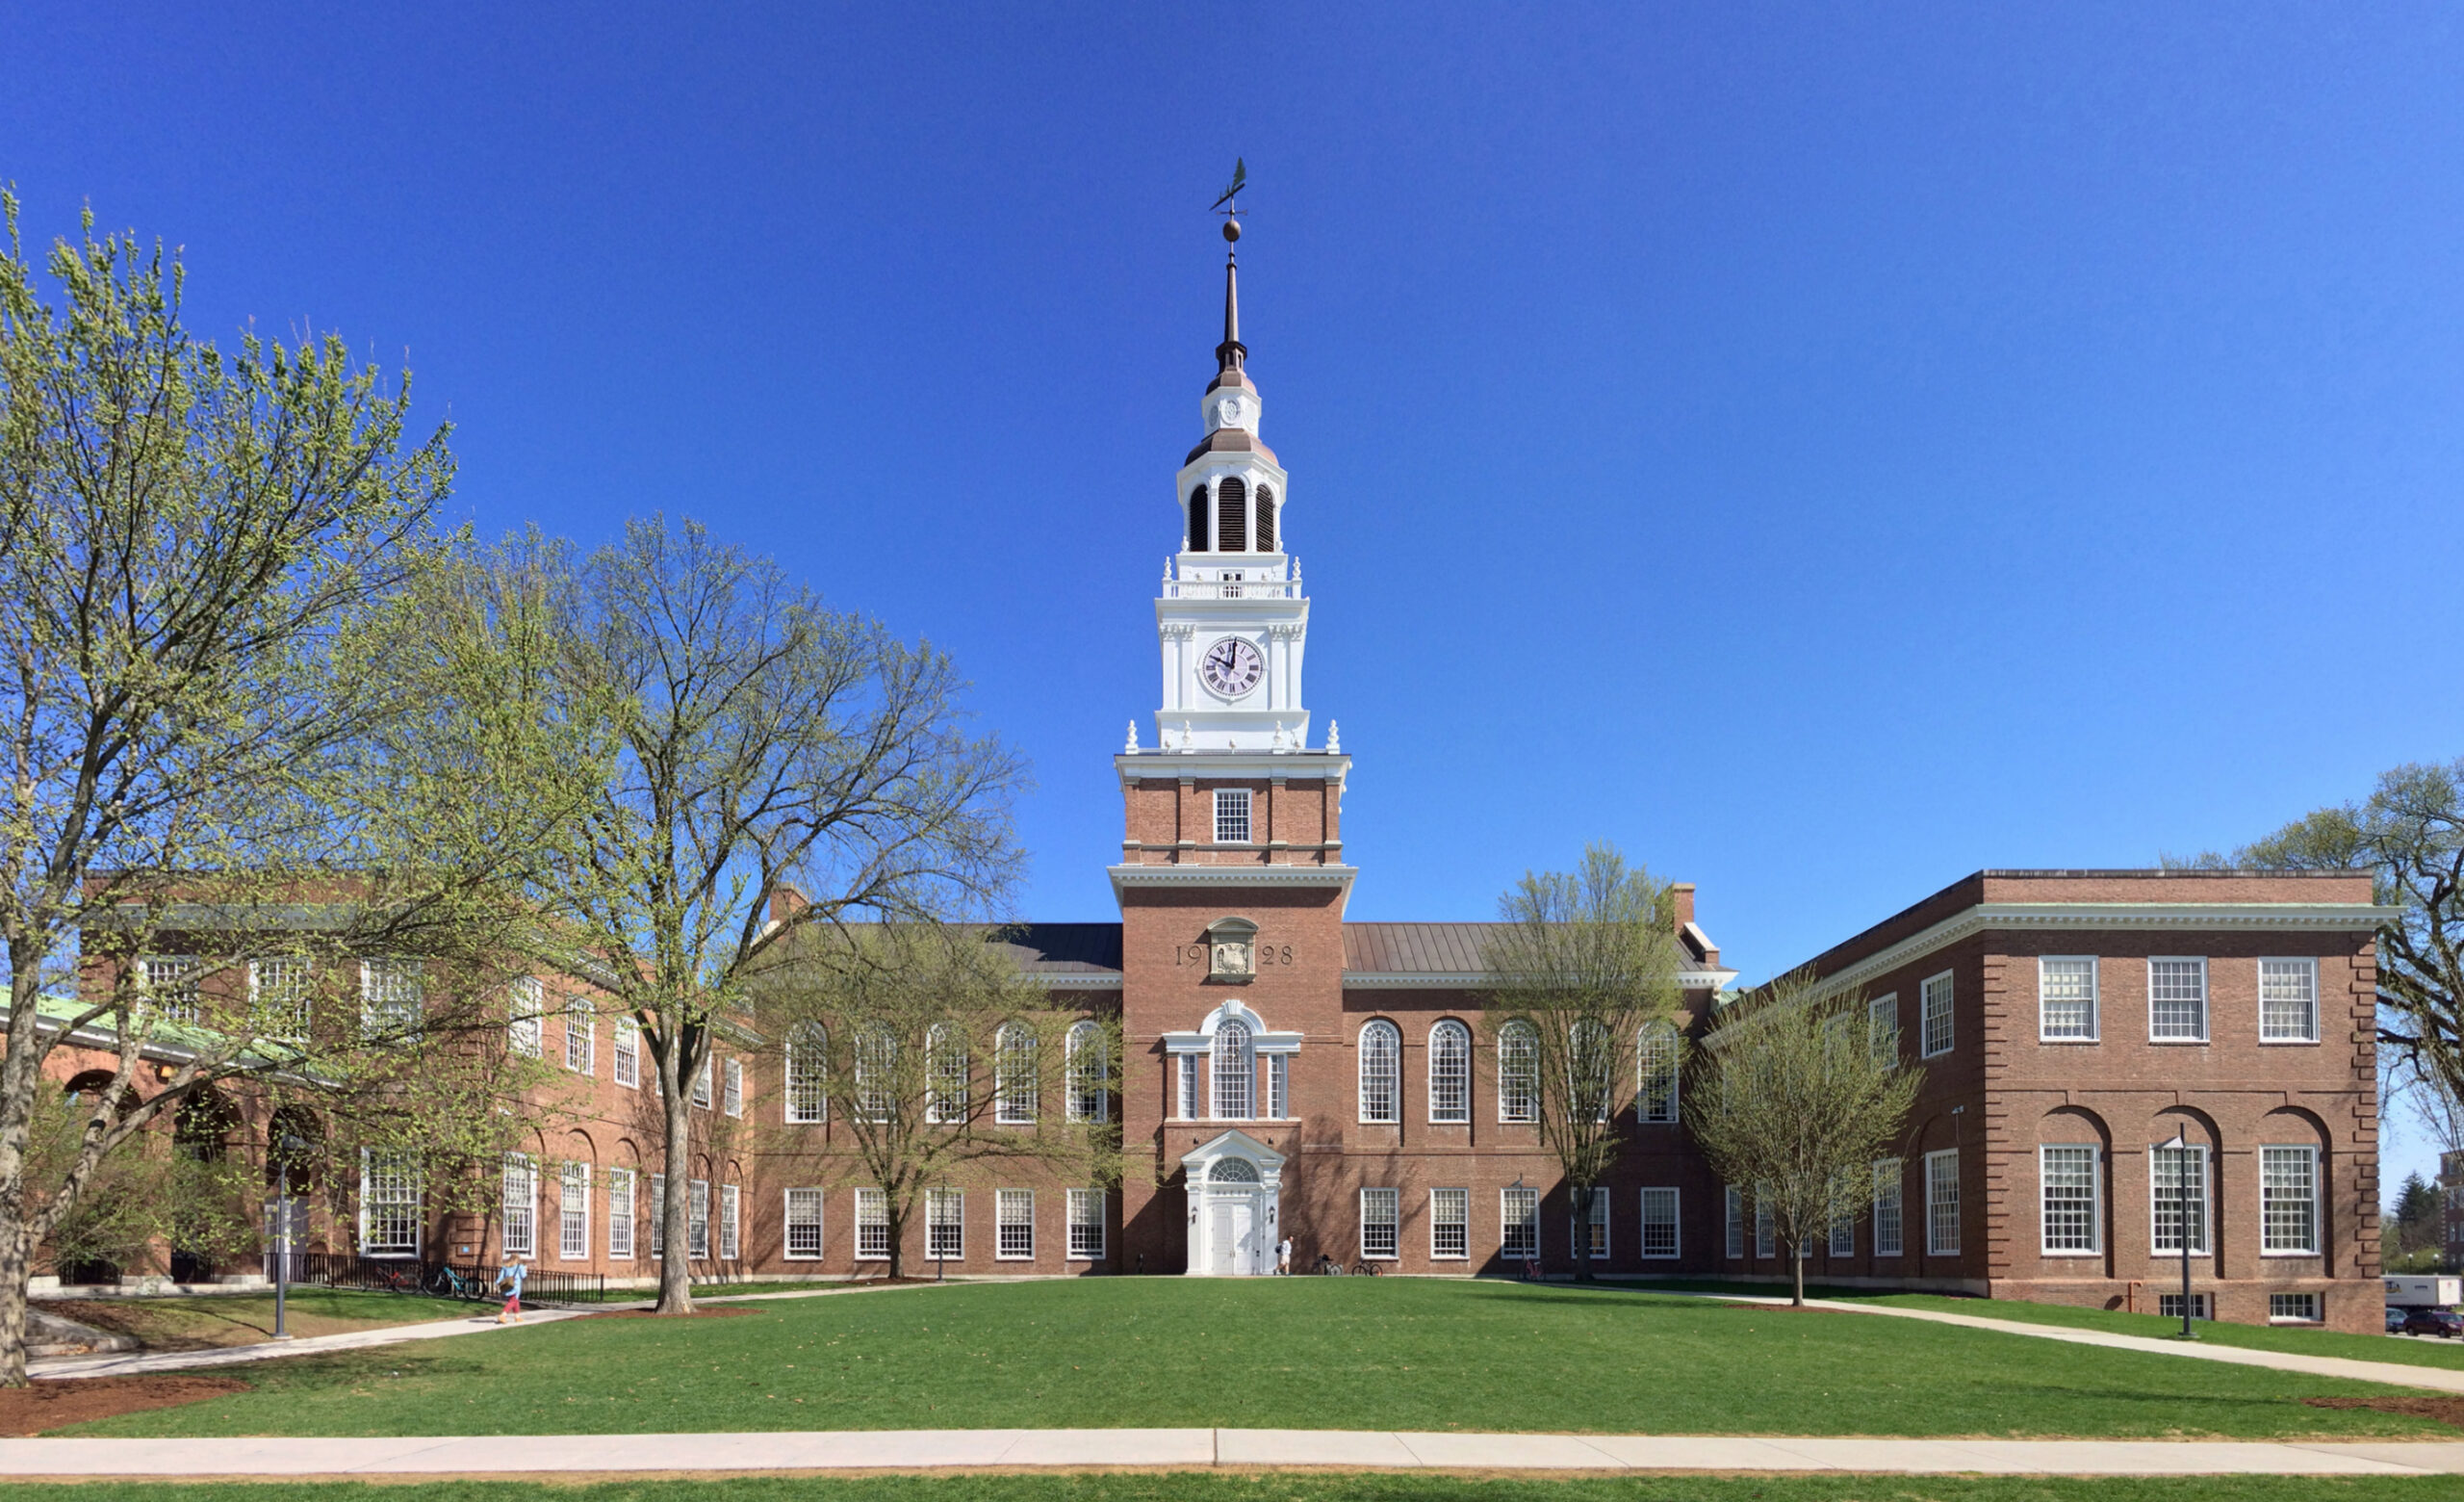
\includegraphics[width=8cm]{imagens/DartmouthCollege.jpg}
\label{Dartmouth College}
\end{figure}

\nocite{college}

	No ano de 1997, o desenvolvimento desta ferramenta veio a demonstrar-se bastante importante, quando o programa de computador \textit{Deep Blue}, desenvolvido pela \ac{ibm}, com sede nos Estados Unidos da América, derrotou o campeão mundial de xadrez Garry Kasparov. Este computador possuía 256 co-processadores, capazes de analisar aproximadamente 200 milhões de posições, por segundo.

	Já uns anos mais tarde, em 2011, um  computador, criado pela mesma empresa, foi colocado á prova, sendo programado para responder a perguntas.

	Posteriormente, no dia 14 de fevereiro de 2016, foi anunciada a \textit{SOPHIA}, um robô com características humanas, com capacidades para produzir cerca de 60 expressões faciais. Este robô, criado por uma empresa de Hong Kong e projetado para aprender e adaptar-se às vivências humanas, consegue realizar reconhecimento facial e processamento de dados.
	
\begin{figure}[H]
\caption{Robô \textit{SOPHIA}}
\centering
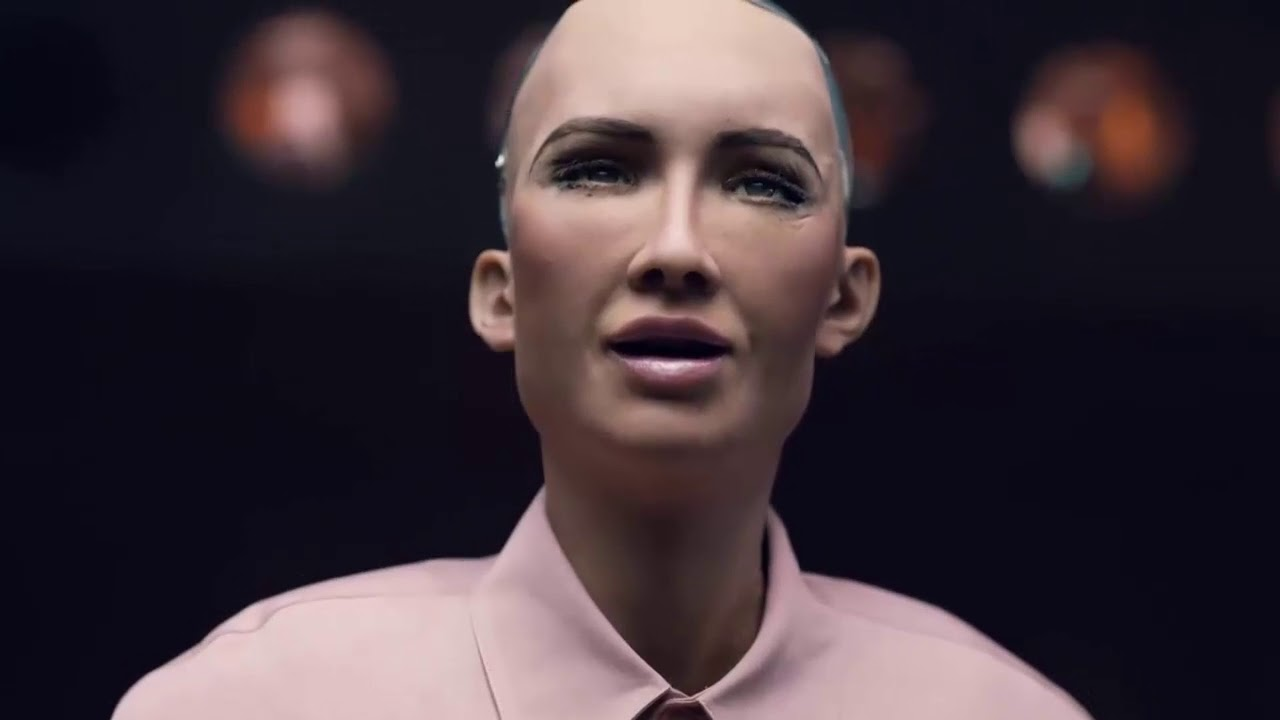
\includegraphics[width=8cm]{imagens/SHOPIA.jpg}
\label{SOPHIA}
\end{figure}

\nocite{sophia}

	Este robô foi o primeiro, na história da tecnologia, a receber cidadania, neste caso, da Arábia Saudita, em outubro de 2017.

	À medida que a \ac{ia} continua a evoluir e se interseta com outros ramos de ciência, como a neurociência e a robótica, novos desafios são criados e, com isso, o seu desenvolvimento nunca está estagnado. \cite{historia}

\subsection{Os tipos de IA}
\label{subsec.os_tipos_de_ia}

	Como já vimos, é inquestionável que a presença da \ac{ia} no nosso quotidiano está a tornar-se cada vez mais vulgar, uma vez que esta permite emular o funcionamento de um ser humano.

	É consensual que a \ac{ia} pode-se dividir em vários grupos, contudo o seu número não o é, já que existe um variado leque de abordagens e técnicas para criar sistemas capazes de realizar tarefas. Por este motivo, em seguida, iremos debrçarmo-nos em quatro divisões: a \ac{ia} fraca, a \ac{ia} forte, o \ac{ml} e a \ac{ia} Quântica.
	
\subsubsection{IA Fraca ou Estreita}
\label{subsubsec.ia_fraca}

	A \ac{ia} fraca refere-se a sistemas computacionais projetados para realizar tarefas específicas. Um exemplo comum deste tipo de \ac{ia} são as \ac{avs}, como a \textit{Siri} e a \textit{Alexa}, que executam comandos ativados por voz, efetuando tarefas simples. Outros exemplos da \ac{ia} estreita incluem algoritmos de recomendação, em plataformas de streaming, como, por exemplo, na \textit{Netflix} e na \textit{Hulu}, e softwares de reconhecimento facial, tais como os usados para desbloquear \textit{smartphones} com biometria facial. \cite{iafraca}
	
\begin{figure}[H]
\caption{\textit{Alexa}}
\centering
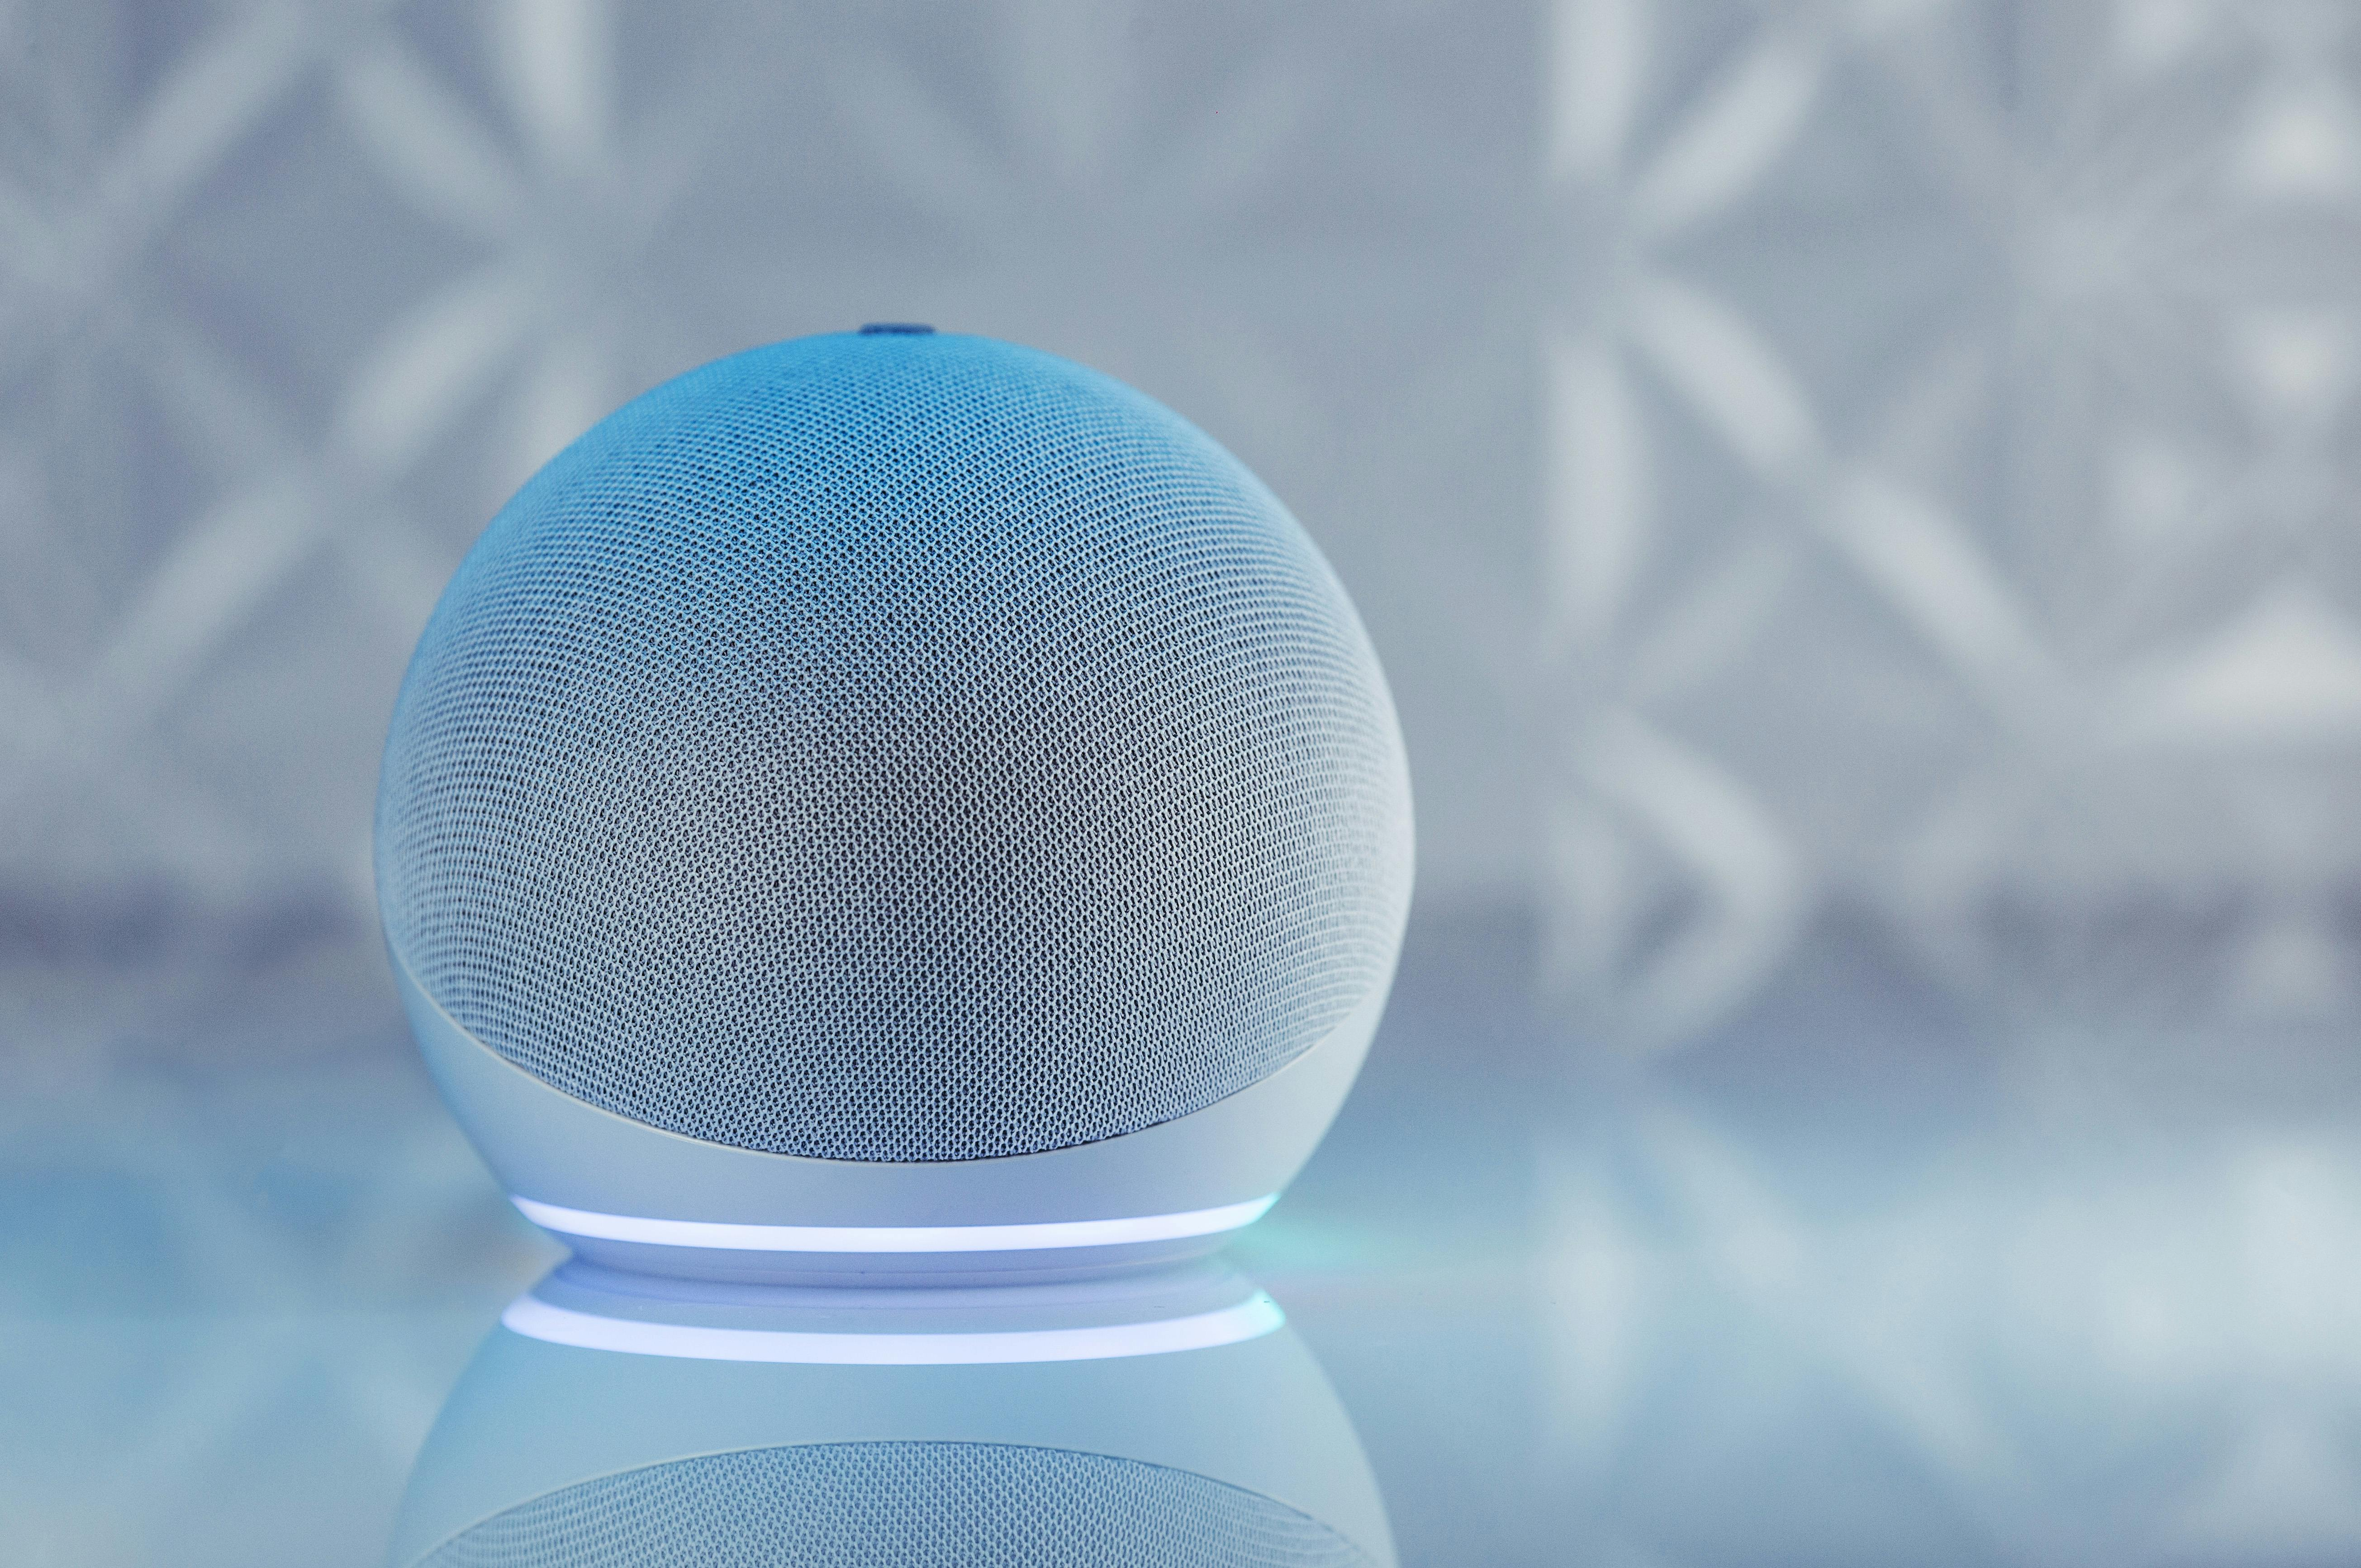
\includegraphics[width=8cm]{imagens/alexa.jpg}
\label{alexa}
\end{figure}

\nocite{alexa}

\subsubsection{IA Forte ou Geral}
\label{subsubsec.ia_forte}

	A \ac{ia} forte representa o culminar da aspiração tecnológica, procurando criar sistemas capazes de replicar a inteligência humana. 

    Este gênero de \ac{ia} está destinado a realizar qualquer tarefa intelectual que um humano consiga realizar, com recurso a consciência e compreensão textual própria. \cite{tipos} \cite{iaforte}

    Embora a \ac{ia} geral represente um campo de pesquisa desafiador e complexo, existem múltiplas aplicações para o uso desta ferramenta. 
    
    Dentro dos seus vastos exemplos de uso, podemos contar com diagnósticos médicos avançados, uma apricabilidade notável que se distingue no recente caso de um sistema de \ac{ia} que consegue detetar cancro da mama com até 5 anos de antecdência. Para este programa, cientistas norte-americanos treinaram o sistema com milhares de mamografias, sendo que, em 2016, foi introduzido ao algoritmo mais de 13,6 mil mamografias. As mulheres envolvidas no estudo foram observadas desde então até 2021, pelo que, com apenas 5 anos de observação, através dos dados extraídos e da sua análise, o sistema de rastreio foi desenvolvido. \cite{cancro} \cite{cancro2}

\subsubsection{Machine Learning}
\label{subsubsec.ml}

	A \ac{ia} revolucionou o mundo da tecnologia e, dentre desse ramo, o \ac{ml} surgiu como uma abordagem fundamental.
	
    O \ac{ml} permite que sistemas computacionais apredam a melhorar o seu desempenho. Através de algoritmos complexos, estes sistemas podem analisar dados, identificar padrões e tomar decisões de forma completamente autónoma.

    Este instrumento permite que os computadores processem grandes quantidades de dados e aprendam com eles, para que realizem tarefas com cada vez mais eficiência. No entanto, a utilização deste \textit{software} levanta questões de ética e privacidade. Por isto, à medida que este evolui, é crucial encontrar-se um equilíbrio entre o potencial inovador e os desafios encontrados, para que seja utilizado de forma responsável, já que o seu futuro promete progressos fascinantes, conforme as fronteiras da \ac{ia} se vão expandindo.
    
\begin{figure}[H]
\caption{\ac{ml} e os conceitos que o rodeiam}
\centering
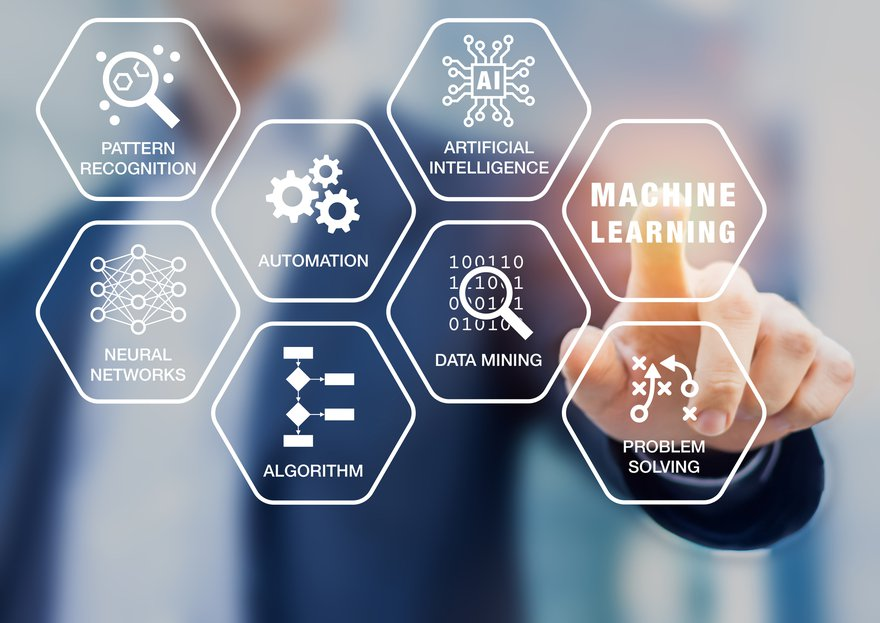
\includegraphics[width=8cm]{imagens/machine_learning.jpg}
\label{machine_learning}
\end{figure}

\nocite{machinelearning}

\subsubsection{IA Quântica}
\label{subsubsec.ia_quantica}

    A \ac{ia} quântica visa explorar a capacidade única de realizar cálculos intensivos. A sua abordagem pode acelerar significativamente a resolução de problemas complexos, como, por exemplo, simulações moleculares. No entanto, a implementação desta prática ainda se encontra em estágios iniciais, enfrentando problemas tecnológicos e de engenharia, pois a necessidade de preservar a coerência quântica representa um obstáculo relevante. \cite{iaquantica}

    À medida que a pesquisa avança neste ramo, estima-se que a \ac{ia} quântica possa vir a alcançar a análise de bases de dados massivas.
    
	O campo do desenvolvimento da \ac{ia} quântica é bastante dinâmico, uma vez que, conforme novas descobertas vão sendo feitas, possibilita a utilização  deste recurso noutros campos.

\section{A rápida explosão da IA}
\label{sec.a_rapida_explosao_da_ia}

	A vertiginosa evolução da \ac{ia} configura um dos acontecimentos mais marcantes na era da tecnologia moderna.
	
	Para chegar ao progresso atual, foram necessários diversos promotores, de entre os quais o aumento da capacidade computacional. A realização de tarefas de forma mais eficiente e a criação de algoritmos mais complexos deve-se ao acréscimo da potência de processamento. Já a aceleração de tarefas desempenhadas pela \ac{ia} foi possível graças à arquitetura de hardware especializado, como, por exemplo, \ac{gpus}. \cite{acrescimo_potencia}
	
\begin{figure}[H]
\caption{Exemplo de \ac{gpus}}
\centering
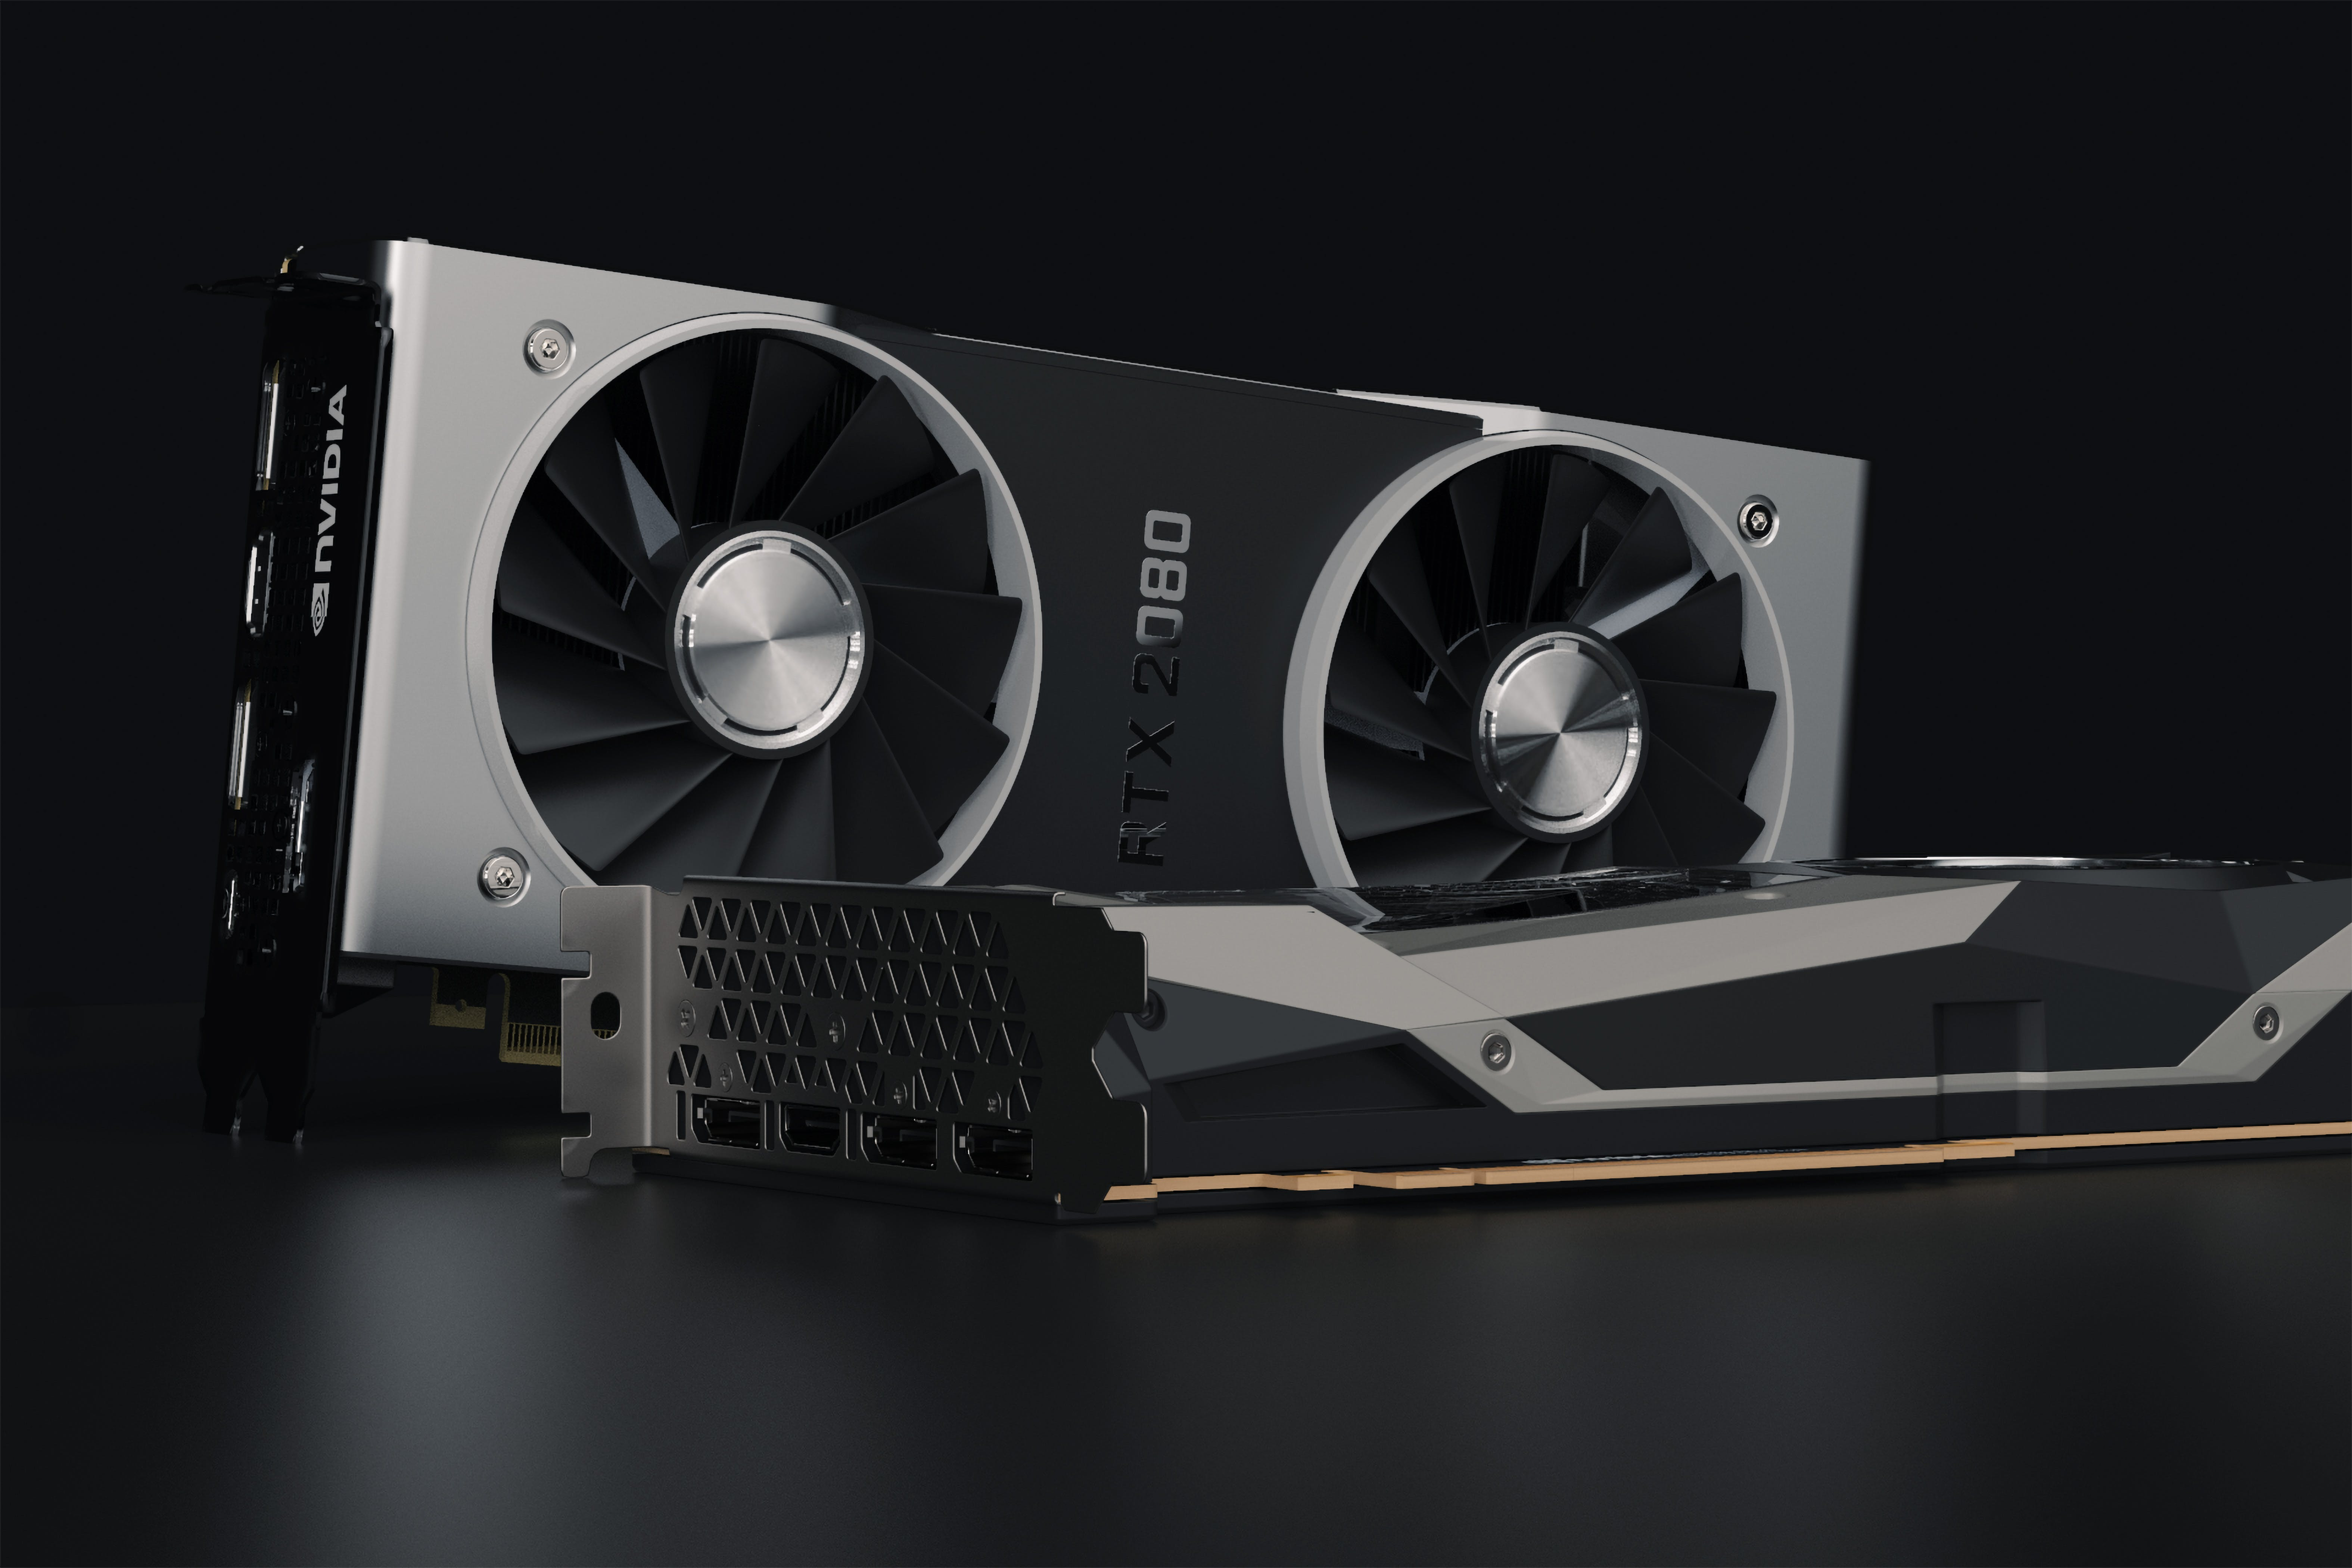
\includegraphics[width=8cm]{imagens/gpu.jpg}
\label{gpu}
\end{figure}

\nocite{gpu}

	As massivas bases de dados disponíveis foram também cruciais para este fenômeno. Os novos sistemas de \ac{ia} são capazes de identificar padrões elaborados devido ao algoritmos de \ac{ml}, cada vez mais desenvolvidos. \cite{machine_learning}

	O avanço e o uso aumentado de tecnologias deste tipo deu-se também, em parte, por conta do interesse e investimento significativo de empresas globais da área tecnológica. Uma "pesquisa com mais de 1.300 CEOs pelo mundo mostra que a grande maioria deles (72\%) considera que o investimento em inteligência artificial (IA) é prioritário [...]", meciona o artigo \textit{"Maioria dos CEOs considera prioritário investimento em inteligência artificial, revela pesquisa"}, publicado em outubro de 2023, pelo Exame. \cite{investimento}
	
	Este interesse monetário suscitou uma competição tecnológica, levando a progressos muito mais rápidos.

\section{Os usos atuais da IA}
\label{sec.os_usos_atuais_da_ia}

	Nos dias de hoje, a \ac{ia} é utilizada em várias secções da sociedade, sendo que, em seguida, iremos explorar quatro exemplos: na saúde, na educação, na assistência virtual e nas finanças.
	
\subsection{Área da Saúde}
\label{subsec.saude}

	Estes programas são um recurso que permitiu variados avanços na área da saúde, sendo usados, por exemplo, em diagnósticos medicinais, uma vez que algoritmos de \ac{dp} (um método que ensina o computador a processar dados de forma semelhante ao cérebro humano) têm a capacidade de analisar imagens médicas e, possivelmente, identificar sinais precoces de doenças. \cite{saude1} \cite{saude2} \cite{saude3}

\begin{figure}[H]
\caption{Posição do \ac{dp} na área da \ac{ia}}
\centering
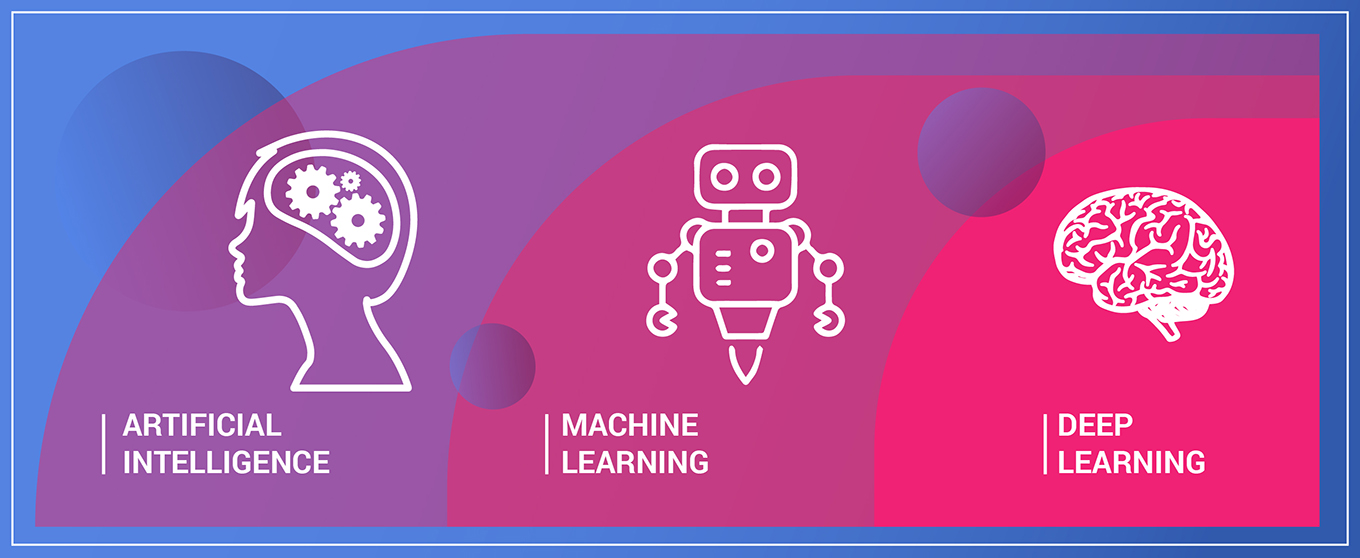
\includegraphics[width=8cm]{imagens/cadeia.jpg}
\label{cadeia}
\end{figure}

\nocite{cadeia}

\subsection{Área da Educação}
\label{subsec.educacao}

	Atualmente, a \ac{ia} é utilizada no campo educacional, de forma a adaptar o processo de aprendizagem individual, onde \ac{itss} modificam, consoante a performance e necessidade de cada estudante, o conteúdo utilizado e testado. Estas ferramentas são capazes ainda de notificar os domínios onde o estudante tem mais dificuldades. \cite{educacao1} \cite{educacao2}
	Alguns exemplos de plataformas de \ac{itss} são: \cite{itss}
	
\begin{itemize}
	\item \textit{Algebra Tutor}, desenvolvido pelo \textit{Pittsburgh Advanced Cognitive Tutor Center}, na Universidade Carnegie Mellon
	\item \textit{SQL-Tutor}, desenvolvido pelo \textit{Intelligent Computer Tutoring Group (ICTG)}, na Universidade de Canterbury
	\item \textit{SmartTutor}, desenvolvido na Universidade de Hong Kong
	\item \textit{ESC101-ITS}, desenvolvido no \textit{Indian Institute of Technology}, em Kanpur

\end{itemize}
	
	Outro possível uso, neste setor, seria a avaliação automática de trabalhos, testes, etc.

\subsection{Assistência Virtual}
\label{subsec.assistencia}

	A \textit{Siri}, \textit{Alexa} e \textit{Google Assistant}, são exemplos de \ac{avs} que utilizam \ac{ia} para as suas funções, fazendo parte do dia-a-dia do cidadão atual, uma vez que são capazes de marcar compromissos, fazer chamadas, responder a mensagens, fazer pesquisas e entregar os resultados mais relevantes, enviar \textit{e-mails}, etc.
	
\begin{figure}[H]
\caption{Exemplos de \ac{avs}}
\centering
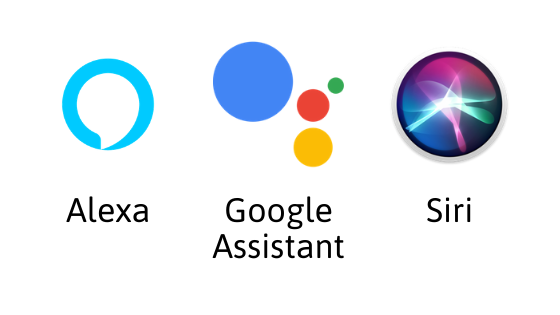
\includegraphics[width=8cm]{imagens/assistants.png}
\label{assistants}
\end{figure}

\nocite{assistants}

	Para o seu funcionamento, utilizam \ac{ml}, tal como \ac{pln}. \cite{av1} \cite{av2}

\subsection{Área Financeira}
\label{subsec.financeira}
	No campo financeiro, sistemas de \ac{ia} são aplicados para detetar atividades suspeitas, prever tendências de mercado e analisar grandes volume de dados. Além disso, conselhos de investimento adaptados ao indivíduo também são possíveis, através de robôs de consultoria, que integram este recurso. \cite{financeiro1} \cite{financeiro2}
	
\begin{figure}[H]
\caption{Usos da \ac{ia} nas finanças e os sistemas neles utilizados}
\centering
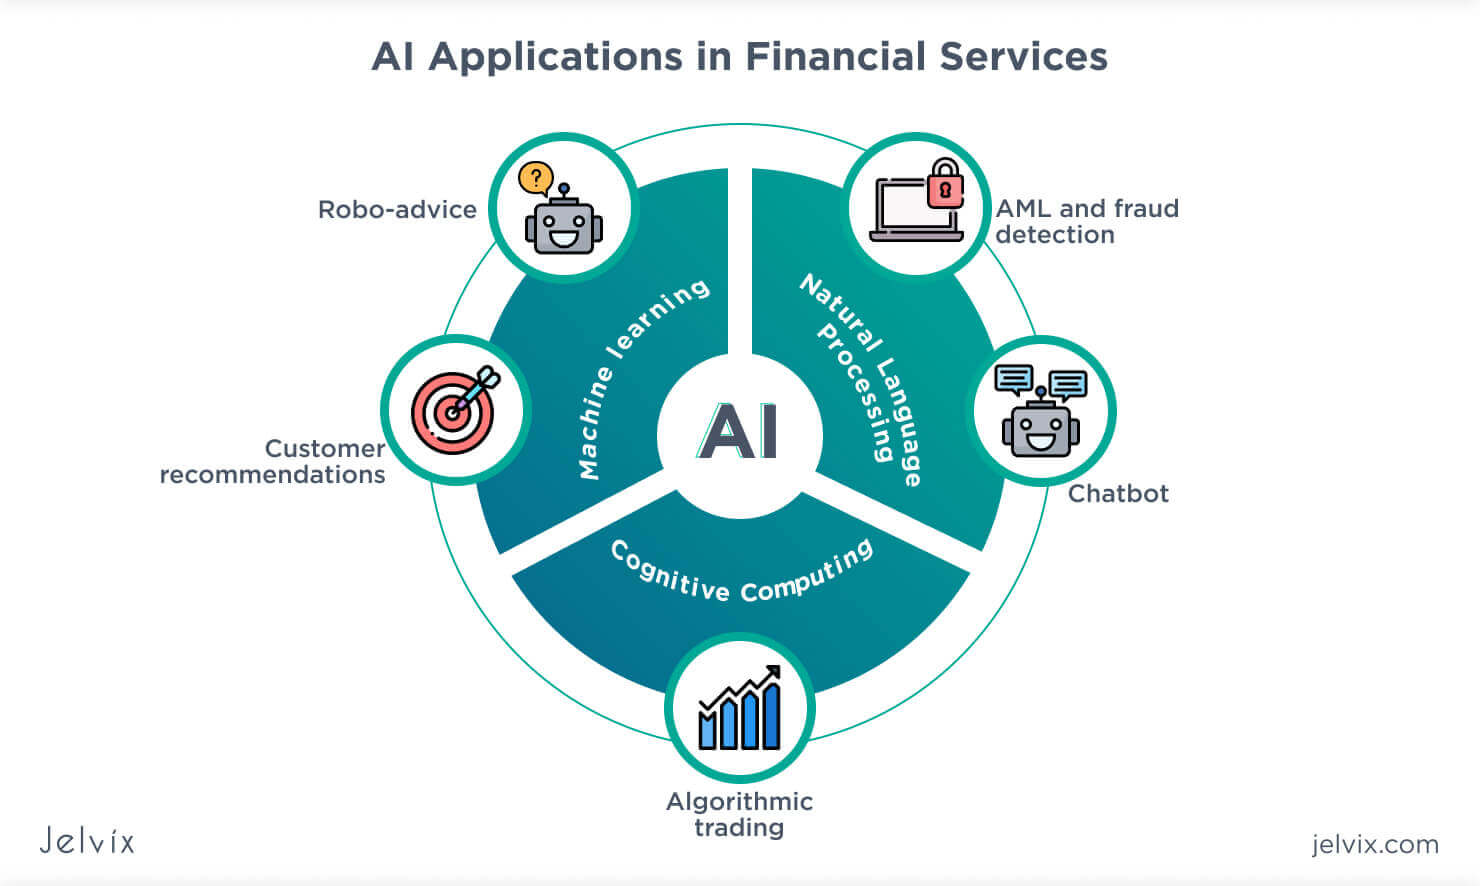
\includegraphics[width=8cm]{imagens/finances.jpg}
\label{finances}
\end{figure}

\nocite{finances}

	Alguns exemplos de plataformas líderes na contribuição de recursos de \ac{ia}, nas áreas financeiras, são: \cite{empresas}

\begin{itemize}
	\item \textit{Salesforce}, uma empresa baseada em gerenciamento de relações com o cliente, que oferece automatização de processos e integração, principalmente para setores financeiros, melhorando a eficiência e a satisfação do cliente
	\item \textit{Brighterion}, uma plataforma de \ac{ia} que analisa dados em tempo real, dando soluções caracterizadas para tomas de decisões importantes, especialmente em setores como finanças e saúde, tendo alta precisão na identificação de fraudes e atenuação de riscos
	\item \textit{Upstart}, uma plataforma de empréstimos que emprega \ac{ml} para analisar uma grande variedade de bases de dados e entregar aos utilizadores empréstimos rápidos e fiáveis
\end{itemize}

\subsection{Vantagens}
\label{subsec.vantagens}

	A \ac{ia}, ao ser utilizada em diversos setores, não apenas traz inovação, mas também oferece um conjunto extenso de vantagens fundamentais. 

	A influência positiva da \ac{ia} é evidente em vários aspetos, tais como:

\begin{enumerate}
	\item \textbf{Otimização de Processos:} A automatização de tarefas repetitivas fomenta a eficiência operacional, apressa a execução deste tipo de atividades e possibilita uma atribuição mais eficaz de recursos.

	\item \textbf{Redução de Erros:} A \ac{ia} contribui consideravelmente para a atenuação de erro humano, assegurando procedimentos mais precisos e fiáveis, o que é bastante importante em setores sensíveis.

	\item \textbf{Processamento de Grandes Volumes de Dados:} A habilidade de trabalhar com massivos conjuntos de dados é um cunho distintivo da \ac{ia}, possibilitando análises mais abrangentes e \textit{insights} importantes, cruciais para a toma de decisões planeadas e informadas.

	\item \textbf{Identificação de Padrões:} Para além de processar grandes bases de dados, a \ac{ia} tem a capacidade de detetar padrões complexos, originando informações relevantes para a toma de decisões informadas, em diversos setores da sociedade, como, por exemplo, a indústria, medicina, finanças, etc.

	\item \textbf{Experiências Personalizadas:} A aptidão da \ac{ia} de aprender com as situações em que é colocada e adaptar-se para tal permite a entrega de interações e/ou respostas caracterizadas em serviços e produtos, aumentando a satisfação do cliente/utilizador e melhorando o relacionamento entre o cliente e a empresa.

	\item \textbf{Sistemas de Recomendação:} A integração de programas de recomendação, baseados em \ac{ia}, torna a experiência do cliente melhor, propiciando sugestões individuais, algo que é especialmente claro em plataformas de streaming, como a \textit{Netflix}, comércio virtual, através de marketing, e redes sociais, como o \textit{Instagram} e o \textit{TikTok}.

	\item \textbf{Detecção de Atividades Suspeitas:} A \ac{ia} executa um papel essencial na identificação de atividades suspeitas, aumentando a segurança em setores nas áreas das finanças e cibersegurança.

	\item \textbf{Reforço da Cibersegurança:} A análise prenunciadora possibilitada pela \ac{ia} é utilizada para prever e prevenir ameaças cibernéticas, garantindo a proteção competente de dados sensíveis e sistemas críticos.

	\item \textbf{Diagnósticos Precisos:} Na área da saúde, a \ac{ia} contribui para diagnósticos médicos mais precisos e, por vezes, a sua descoberta com mais antecedência e tratamentos caracterizados, aproveitando dados clínicos para dar abordagens mais eficazes.

	\item \textbf{Avanços na Pesquisa Médica:} A análise de dados genômicos, promovida pela \ac{ia}, está a conduzir progressos significativos na pesquisa medicinal, acelerando descobertas e ajudando ao movimento da medicina personalizada.
\end{enumerate}

	Estas são apenas algumas, das muitas, maneiras como a \ac{ia} transforma, de forma positiva, várias partes do mundo atual, destacando-se não apenas pela eficiência, mas também pela inovação nos diversos campos, moldando a era da \ac{ia} de maneiras nunca antes vistas.

\subsection{Desvantagens}
\label{subsec.desvantagens}

	Embora a \ac{ia} ofereça as vantagens descritas anteriormente, e muitas outras, é importante mencionar as desvantagens que lhe estão associadas.

\subsubsection{Impacto no Emprego}
\label{subsubsec.emprego}

	Um dos maiores desafios no avanço da \ac{ia} é o potencial impacto no emprego. À medida que os sistemas automatizados e os algoritmos de aprendizagem automática se tornam mais sofisticados, alguns empregos tradicionais podem ser substituídos, perdendo-se-os. Empregos que antigamente eram dados como certos, como, por exemplo, designers gráficos, podem, agora, ser trocados por programas projetados para essas funções.

\subsubsection{Vieses nos Algoritmos}
\label{subsubsec.algoritmos}
	
	Os algoritmos de \ac{ia} podem herdar preconceitos existentes nos seus dados de treino. Se os dados usados para treinar esses algoritmos forem tendenciosos, os resultados poderão refletir e amplificar esses preconceitos. Isto pode levar à discriminação em áreas como o recrutamento, o crédito e a justiça criminal, e agravar a desigualdade social. \cite{vieses} \cite{vieses2}

\subsubsection{Privacidade e Segurança dos Dados}
\label{subsubsec.privacidade}

	A utilização da \ac{ia} exige a recolha e tratamento de dados pessoais. Isto levanta preocupações significativas sobre privacidade e segurança de dados. Se não forem implementadas proteções fortes, estes sistemas podem representar
uma ameaça à privacidade pessoal, com consequências potencialmente adversas.

\subsubsection{Falta de Transparência}
\label{subsubsec.transparencia}

	Muitos algoritmos funcionam como caixas pretas, dificultando a compreensão completa das suas tomas de decisões. A falta de transparência nos processos de decisão pode levar à desconfiança entre os utilizadores. \cite{transparencia}

\subsubsection{Desafios Éticos}
\label{subsubsec.etica}

	A utilização da \ac{ia} traz desafios éticos, como a autonomia das máquinas, a responsabilidade pela tomada de decisões automatizadas e a necessidade de definir limites éticos. A inovação deve ser equilibrada, com considerações éticas, para maximizar os benefícios e minimizar os riscos. \cite{desafios1} \cite{desafios2}

\section{O que esperar a curto e médio prazo?}
\label{sec.o que esperar}

	O desenvolvimento da \ac{ia} nos últimos anos levantou questões relevantes sobre o que podemos esperar a curto e médio prazo, pelo que, em seguida, iremos explorar tendências e perspetivas futuras para a \ac{ia}. \cite{prazo1} \cite{prazo2}

\subsection{Avanços Tecnológicos Emergentes}
\label{subsec.avançostecno}

	Melhorar os algoritmos de \ac{ml} e aumentar o poder computacional ajudará a criar sistemas mais eficientes e inteligentes.
	Espera-se que a integração de tecnologias como o \ac{dp} melhore a capacidade da \ac{ia} de compreender e resolver tarefas complexas. \cite{emergentes1} \cite{emergentes2}

\subsection{Aplicações Práticas em Diversos Setores}
\label{subsec.aplicacoes}

A utilização da \ac{ia} em vários setores da sociedade é uma tendência predominante que deverá continuar a curto e médio prazo. Setores como saúde, finanças, educação e manufatura estão a adotar soluções baseadas em \ac{ia}, para aumentar a sua eficiência operacional, porém esta expansão deverá passar para além destes setores. \cite{praticas1} \cite{praticas2}

\begin{figure}[H]
\caption{Exemplos de setores onde a expansão da \ac{ia} poderá acontecer}
\centering
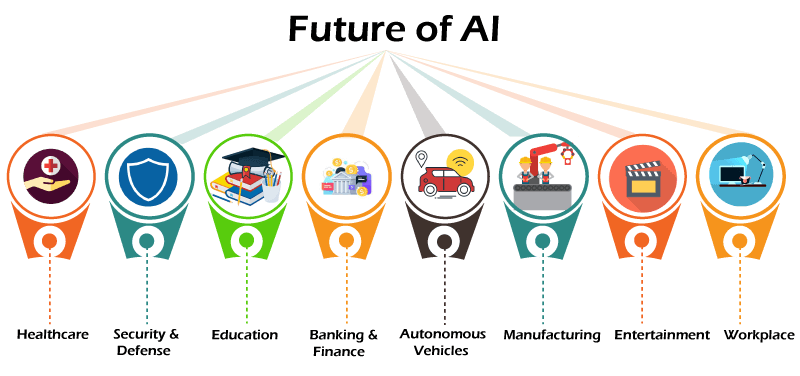
\includegraphics[width=8cm]{imagens/future.png}
\label{future}
\end{figure}

\nocite{future}

\subsection{Desafios Éticos e Regulamentares}
\label{subsec.desafios}

	À medida que a \ac{ia} se torna cada vez mais integrada na vida quotidiana, surgem desafios éticos e dilemas regulamentares. O estabelecimento de padrões éticos para o desenvolvimento e utilização do recurso torna-se imperativo. As preocupações relativas à privacidade, segurança e preconceitos algorítmicos exigirão atenção significativa, tanto da sociedade como dos decisores políticos. \cite{etica}

\subsection{Impacto nas Dinâmicas do Mercado de Trabalho}
\label{subsec.impacto}

	A proliferação da tecnologia de \ac{ia} suscitou apreensão quanto ao impacto no mercado de trabalho. A automatização de tarefas pode exigir modificações nas competências dos trabalhadores, sublinhando a importância da implementação de iniciativas de requalificação, para facilitar uma transição perfeita à crescente prevalência da \ac{ia}. \cite{emprego}

\subsection{Inovações Contínuas e Colaboração Internacional}
\label{subsec.inovacoes}

	A cooperação internacional é imperativa para a disseminação da \ac{ia}. Dado que os desafios e as perspetivas se estendem para além das fronteiras nacionais, a colaboração entre nações, instituições e universidades é vital para o progresso e para garantir que a \ac{ia} sirva para a melhoria da humanidade como um todo.

\chapter{Análise}
\label{chap.analise}

	Na \autoref{chatgpt} observamos a interface do \textit{ChatGPT}, uma plataforma que utiliza \ac{ml} para analisar os pedidos e informações dadas pelos seus utilizadores, de forma a entregar as melhores repostas possíveis.	
	
	Como podemos observar, pela \autoref{Crescimento da receita de IA em milhares de dolares ao longo dos anos}, a análise do gráfico demonstra a receita, em milhares de dólares (US), do mercado de \ac{ia}, ao longo dos últimos anos. O crescimento é exponencial e espera-se que em 2025 a receita seja em mais de duas vezes a de 2022.
	
	A \autoref{Dartmouth College} é uma fotografia do campus onde foi criado o primeiro e tão importante programa de \ac{ia}, denominado \textit{Logic Theorist}, enquanto que, na \autoref{SOPHIA}, é possível observar o primeiro robô, na história, a obter a nacionalidade de um país.
	
	Na \autoref{alexa} vê-se uma das \ac{avs} existentes atualmente, a \textit{Alexa}.
	
	A \autoref{machine_learning} demonstra os conceitos que rodeiam o \ac{ml}: \textit{pattern recognition}, \textit{neural networks}, \textit{automation}, \textit{algorithm}, \textit{artificial inteligence}, \textit{data mining} e \textit{problem solving}. Alguns destes tópicos foram abordados em variadas posições do relatório.
	
	Na \autoref{gpu} encontra-se um exemplo de uma \ac{gpus}, peça que é responsável, em parte, pela aceleração de tarefas desempanhadas pela \ac{ia}.
	
	A \autoref{cadeia} demonstra o posicionamento do DP na cadeia de conceitos que envolvem a \ac{ia}.
	
	Exemplos de \ac{avs}, mais especificamente, a \textit{Siri}, a \textit{Google Assistant} e a \textit{Alexa}, estão presentas na \autoref{assistants}.
	
	Na \autoref{finances} são esquematizados os sistemas, relacionados com \ac{ia}, que são, maioritariamente, utilizadas na área das finanças. Dentro do conceito de \ac{ia} podemos considerar os subconceitos: \ac{ml}, \ac{pln} e computação cognitiva. Dentro de cada um destes subconceitos são dados exemplos de como eles podem ser aplicados.
	
	Por fim, na \autoref{future} tem-se um esquema com saúde, segurança e defesa, educação, finanças, veículos de condução autónoma, manufaturação, entretenimento e mercado de trabalho como exemplos de para que setores a \ac{ia} poderá expandir-se no futuro.

\chapter{Conclusão}
\label{chap.conclusao}
	Em conclusão, desde as suas raízes conceituais, nos escritos de Alan Turing, até aos avanços contemporâneos, temos testemunhado uma notável evolução no desenvolvimento desta tecnologia. A \ac{ia} não é apenas uma ferramenta revolucionária, mas sim "a capacidade de uma máquina reproduzir competências humanas, como é o caso do raciocínio crítico, a aprendizagem, o planeamento e a criatividade" (\textit{"O que é a inteligência artificial e como funciona?"}, publicado pelo Parlamento Europeu, em 2020), algo que antes seria considerado possíevl exclusivamente ao Homem.
	
	Contudo, esta revolução não é toda um mar de rosas, uma vez que questões de ética e privacidade estão no topo das preocupações, quando se fala sobre o uso desta
tecnologia, e requerem uma atenção cuidadosa. No entanto, a \ac{ia} oferece
oportunidades vastas e inexploradas até aos dias de hoje, onde a criatividade é
o limite. \cite{lei}

	Por fim, neste cenário de rápida evolução, o resultado da \ac{ia} é tanto um reflexo das capacidades humanas quanto uma janela para o futuro. É o nosso papel
orientar o seu desenvolvimento de maneira responsável, garantindo que esta
tecnologia é um catalisador para um futuro promissor.

\chapter*{Contribuições dos autores}

	Ambos os autores participaram da escrita da introdução.
	
	A \ac{mm} escreveu o resumo e parte da introdução. Esta autora também pesquisou e desenvolveu sobre a rápida explosão da \ac{ia} e os usos atuais da \ac{ia}. A \ac{mm} escreveu sobre as vantagens e desvantagens do uso de \ac{ia}, tal como sobre o que esperar a curto e médio prazo.
	
	O \ac{fp} escreveu sobre a \ac{ia}, o que ela é e a sua história. Este autor também redigiu sobre os tipos de \ac{ia}. O \ac{fp} contribuiu com a análise, tal como com a conclusão.
	
	Por fim, a \ac{mm} reviu todo o trabalho, de forma a verificar que não existem erros.\\

\autores : 50\%, 50\%\\


\chapter*{Acrónimos}
\begin{acronym}
\acro{ia}[IA]{Inteligência Artificial}
\acro{avs}[AVs]{Assistentes Virtuais}
\acro{gpus}[GPUs]{Unidades de Processamento Gráfico}
\acro{ml}[ML]{\textit{Machine Learning}}
\acro{dp}[DP]{\textit{Deep Learning}}
\acro{itss}[ITSs]{\textit{Intelligent Tutoring Systems}}
\acro{pln}[PLN]{Processamento de Linguagem Natural}
\acro{ibm}[IBM]{\textit{International Business Machines Corporation}}
\acro{ctr}[CTR]{\textit{Computing Tabulating Recording Company}}
\acro{risc}[RISC]{\textit{Reduced Instruction Set Computing}}
\acro{mm}[MM]{Matilde Marabuto}
\acro{fp}[FP]{Francisco Pedreiras}
\end{acronym}


\printbibliography

\appendix
\chapter{IBM}
\label{ibm}

    A \ac{ibm} é uma empresa com sede nos Estados Unidos da América, fundada por Charles Ranlett Flint e Thomas John Watson, a 16 junho de 1911, sendo esta uma das mais influentes no mundo da tecnologia.
    
    Esta empresa possui cerca de 280 mil funcionários e é caracterizada por uma notável capacidade de adaptação e inovação contínua. 
    
    A história desta empresa começou com a criação da \ac{ctr}, mais tarde renomeada para \ac{ibm}, refletindo o objetivo da empresa de se tornar uma líder em tecnologia e processamento de dados.
    
    A década de 1950 ficou marcada como um ponto de viragem, com a introdução do \ac{ibm} 701, o primeiro computador científico de grande escala do mundo. Nos anos seguintes, a empresa consolidou-se no mercado, criando computadores de médio porte, como, por exemplo, o \ac{ibm} 1401, focado em aplicações comerciais.

    Já a década de 1980 trouxe grandes mudanças. Com a \ac{ibm} a mover-se na direção da criação de serviços e \textit{software}, surgiu a criação do sistema operativo OS/2 e o desenvolvimento da arquitetura \ac{risc}. Contudo, a empresa emfrentou desafios e teve de adptar-se, uma vez que, em 1993, a esta anunciou prejuízos históricos, o que originou um período de reestruturação e, mais uma vez, mudança de foco.

    A mundança de século originou uma transformação nesta empresa, que se concentrou, cada vez mais, em serviços e soluções de \textit{software}. 

    Nos ultímos anos, a \ac{ibm} tem desempenhado um papel fundamental na promoção de tecnologias, como a \ac{ia} e a computação quântifca, incluindo o computador \ac{ibm} Watson, que venceu contra humanos no jogo \textit{Jeopardy}. O desenvolvimento da sua tecnologia em computação quântica ainda está no início, mas visa revolucionar a capacidade de processamento de dados.

    Em resumo, a \ac{ibm} é uma empresa que evoluiu continuamente, ao longo da sua história centenária, mantendo-se firme na inovação tecnológica, prevendo tendências emergentes, o que demostra a visão e o compromisso da empresa.
    
\end{document}